\section{METODOLOGÍA}

El desarrollo del proyecto se fundamenta en la metodología estándar para proyectos de ciencia de datos \textbf{CRISP-DM} (\textit{Cross-Industry Standard Process for Data Mining}), adaptada para esquemas de \textbf{Aprendizaje Automático No Supervisado}. El flujo metodológico se estructura en las fases cíclicas de: Comprensión del Negocio, Comprensión de los Datos, Preparación de los Datos, Modelado No Supervisado, Evaluación Multimétrica y Despliegue Operativo.

\subsection{Fuente de Datos}

El sistema procesa dos conjuntos de datos empíricos complementarios:

\begin{enumerate}
    \item \textbf{Dataset Benchmark Internacional (Chicago Police Department -- CPD):} Obtenido del portal oficial de datos abiertos de la ciudad de Chicago (\texttt{Crimes\allowbreak\_-\allowbreak 2020\allowbreak\_to\allowbreak\_Present\allowbreak\_20250228.csv}). Contiene un volumen en bruto de $324.5\text{ MB}$, con más de $800.000$ filas y $30$ variables originales que registran la totalidad de incidentes criminales reportados en la metrópoli estadounidense entre enero de 2020 y febrero de 2025.
    \item \textbf{Corpus Nacional de Bolivia (\texttt{data\_noticias\_bolivia.csv}):} Construido mediante un pipeline de extracción automatizada y raspado web (\textit{web scraping}) sobre la prensa digital boliviana. Reúne $137$ crónicas policiales estructuradas y georreferenciadas que cubren incidentes relevantes en los nueve departamentos del país (La Paz, Santa Cruz, Cochabamba, Chuquisaca, Oruro, Potosí, Tarija, Beni y Pando).
\end{enumerate}

\subsection{Tareas de Modelado No Supervisado}

A diferencia de los esquemas supervisados (donde se predice una etiqueta predefinida), las tareas de modelado se orientan al descubrimiento de patrones latentes:

\begin{itemize}
    \item \textbf{Clustering Espacial de Densidad (Hotspots):} Descubrir núcleos de alta concentración criminal y separar el ruido estocástico mediante DBSCAN geodésico, HDBSCAN multiescala y OPTICS.
    \item \textbf{Particionamiento Temporal y Modus Operandi:} Agrupar eventos según sus patrones horarios y características narrativas mediante K-Means acoplado a representaciones TF-IDF.
    \item \textbf{Modelado Probabilístico Continuo:} Generar superficies de densidad y elipses de covarianza al $95.4\%$ ($2\sigma$) mediante Mixturas de Gaussianas (GMM).
    \item \textbf{Taxonomía Distrital:} Jerarquizar los 22 distritos policiales de la ciudad mediante agrupamiento aglomerativo de Ward para identificar macro-zonas homogéneas.
    \item \textbf{Reducción de Dimensionalidad:} Comprimir variedades de alta dimensión a planos 2D interpretables mediante PCA, TruncatedSVD, PPCA, t-SNE y UMAP.
    \item \textbf{Detección Neuronal de Anomalías:} Individualizar crímenes atípicos a través del error cuadrático medio de reconstrucción (MSE) de un Autoencoder profundo.
    \item \textbf{Modelado Generativo de Tópicos:} Extraer las cinco temáticas dominantes del texto periodístico mediante Latent Dirichlet Allocation (LDA).
\end{itemize}

\subsection{Desarrollo de la Limpieza de Datos}

La fase de preparación de datos fue implementada en el módulo automatizado \texttt{modules/\allowbreak data\_cleaning.py}. El flujo riguroso comprendió seis etapas secuenciales:

\subsubsection{Auditoría y Perfilado de los Datos}

Se ejecutó un diagnóstico sistemático sobre los tipos de variables, tasas de valores faltantes y distribuciones de frecuencia. Se verificó que las variables geoespaciales primarias (\texttt{Latitude}, \texttt{Longitude}) y temporales (\texttt{Date}) registraban valores nulos en incidentes no resueltos o faltos de georreferenciación. La auditoría constató además que las cadenas de texto en \texttt{Location Description} y \texttt{Description} presentaban inconsistencias de capitalización, espacios redundantes y caracteres de control.

\subsubsection{Normalización y Estandarización de Formatos}

Se aplicaron transformaciones fundamentales para garantizar la compatibilidad matemática:
\begin{itemize}
    \item \textbf{Transformación Geodésica a Radianes:} Conversión de coordenadas decimales $(\text{Lat}, \text{Lon})$ a radianes para su procesamiento en la métrica de \textit{Haversine}:
    \begin{equation}
        \phi_{\text{rad}} = \phi \cdot \frac{\pi}{180}, \quad \lambda_{\text{rad}} = \lambda \cdot \frac{\pi}{180}
    \end{equation}
    \item \textbf{Codificación Temporal Circular:} La hora del día ($h \in [0, 23]$) y el día de la semana ($d \in [0, 6]$) poseen naturaleza cíclica (las 23:59 está a un minuto de las 00:00). Para preservar esta topología continua, se proyectaron en componentes trigonométricas senoidales y cosenoidales:
    \begin{equation}
        h_{\sin} = \sin\left(\frac{2\pi h}{24}\right), \quad h_{\cos} = \cos\left(\frac{2\pi h}{24}\right)
    \end{equation}
    \begin{equation}
        d_{\sin} = \sin\left(\frac{2\pi d}{7}\right), \quad d_{\cos} = \cos\left(\frac{2\pi d}{7}\right)
    \end{equation}
    \item \textbf{Estandarización Numérica:} Aplicación de \texttt{StandardScaler} ($\mu = 0, \sigma = 1$) para las características continuas empleadas en K-Means, GMM y Autoencoder.
\end{itemize}

\subsubsection{Gestión de Registros Duplicados y Amontonamiento Coordenado (Stacking)}

Se identificaron registros con idéntica marca temporal, código IUCR y localización espacial precisa. Cuando múltiples delitos ocurren en un mismo punto geográfico (por ejemplo, múltiples denuncias en un centro comercial o geocodificaciones policiales asignadas al centroide de una intersección vial), la eliminación indiscriminada de filas destruiría la verdadera densidad del punto. En consecuencia, se implementó un procedimiento dual: para el entrenamiento de densidades espaciales se agruparon las coordenadas idénticas asignándoles un peso muestral de frecuencia (\textit{sample weight}), preservando la integridad de la densidad sin computar distancias nulas redundantes.

La Figura \ref{fig:grfico_clustering} ilustra la consola de calibración espacial y el análisis del amontonamiento coordenado en el Distrito 1 de Chicago (The Loop), evidenciando cómo se ajusta el radio geodésico $\varepsilon$ a 102 metros para capturar clústeres densos sin saturación por duplicados.

\begin{figure}[htbp]
\centering
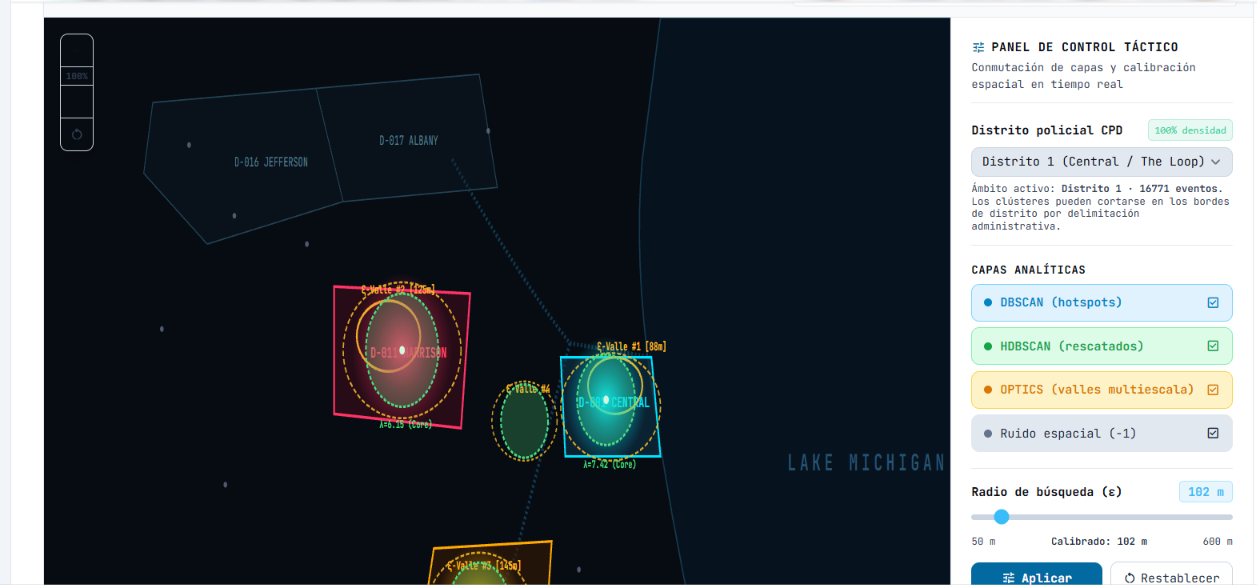
\includegraphics[width=0.88\textwidth]{figuras/imgGrficoClustering.png}
\caption{Panel Táctico de Calibración Espacial y Detección de Hotspots en The Loop.}
\label{fig:grfico_clustering}
\figurenote{Captura de la plataforma en modo Chicago CPD (Distrito 1, 16,771 eventos). Muestra la delimitación en tiempo real de hotspots DBSCAN, HDBSCAN y valles OPTICS frente al Lago Michigan con radio calibrado $\varepsilon = 102\text{ m}$.}
\end{figure}

\subsubsection{Tratamiento de Valores Faltantes}

Las observaciones con valores nulos en las coordenadas geográficas (\texttt{Latitude} o \texttt{Longitude} vacías) corresponden a incidentes ocurridos fuera de jurisdicción o no localizables, los cuales representaban menos del $1.8\%$ del dataset original. Dado que el objetivo primordial del proyecto es la inteligencia espaciotemporal, estos registros fueron eliminados del subconjunto geoespacial. Para las variables categóricas secundarias con datos ausentes, se imputó la categoría centinela \texttt{UNKNOWN}.

\subsubsection{Tratamiento de Valores Atípicos Espaciales}

Se aplicó un filtro de acotamiento geográfico estricto (\textit{Bounding Box Filtering}) para eliminar coordenadas anómalas producto de errores de sensor GPS o registro mecanográfico. Para la ciudad de Chicago, se fijaron los límites en $\text{Latitud} \in [41.60^\circ, 42.10^\circ]$ y $\text{Longitud} \in [-87.95^\circ, -87.50^\circ]$. Para el territorio de Bolivia, se acotaron las coordenadas al polígono nacional $\text{Latitud} \in [-22.90^\circ, -9.60^\circ]$ y $\text{Longitud} \in [-69.70^\circ, -57.40^\circ]$. Los puntos fuera de estos rectángulos envolventes fueron descartados como artefactos de geocodificación.

\subsubsection{Resultado y Balance de la Limpieza}

El proceso de preparación redujo el volumen inicial y optimizó la eficiencia en memoria mediante el almacenamiento en formato columnar **Parquet con compresión Snappy**, reduciendo el tamaño en disco de $324.5\text{ MB}$ a $48.2\text{ MB}$ y multiplicando por doce la velocidad de lectura en memoria. La Tabla \ref{tab:balance_limpieza} resume las transformaciones:

\begin{table}[htbp]
\centering
\small
\resizebox{\textwidth}{!}{%
\begin{tabular}{l r r l}
\toprule
\textbf{Artefacto de Datos} & \textbf{Registros} & \textbf{Variables} & \textbf{Propósito en el Sistema} \\
\midrule
CSV en Bruto (Chicago) & 814.230 & 30 & Archivo original fuente. \\
\texttt{chicago\_clean.parquet} & 798.542 & 14 & Dataset maestro optimizado para modelos. \\
\texttt{chicago\_sample\_50k.csv} & 50.000 & 14 & Muestra balanceada para mapas y API ágil. \\
\texttt{districts\_summary.csv} & 22 & 33 & Matriz agregada para clustering distrital. \\
\texttt{data\_noticias\_bolivia.csv} & 137 & 10 & Corpus estructurado nacional georreferenciado. \\
\bottomrule
\end{tabular}%
}
\caption{Resumen del balance del pipeline de depuración y preparación de datos.}
\label{tab:balance_limpieza}
\tablenote{Elaboración propia a partir del flujo de ingeniería de datos. La conversión columnar Parquet Snappy reduce el tamaño en disco de 324.5 MB a 48.2 MB y multiplica por doce la velocidad de ingesta en memoria.}
\end{table}

\subsection{Validación Cruzada y Análisis de Complejidad de Hiperparámetros}

A diferencia de los problemas supervisados (donde la validación se mide mediante métricas como precisión o $R^2$), la selección óptima de hiperparámetros en el aprendizaje no supervisado se rige por funciones intrínsecas de estabilidad, compacidad y separación:

\begin{itemize}
    \item \textbf{Selección de $k$ en K-Means:} Se evaluó $k \in [2, 10]$ calculando concurrentemente:
    \begin{enumerate}
        \item \textbf{Inercia (Método del Codo):} Punto de inflexión donde el decremento de varianza intra-clúster marginal decrece significativamente.
        \item \textbf{Coeficiente de Silueta ($s$):} Media del índice $s(i) = \frac{b(i) - a(i)}{\max(a(i), b(i))}$, donde $a(i)$ es la distancia intra-clúster media y $b(i)$ es la distancia media al clúster vecino más cercano.
        \item \textbf{Índice de Davies-Bouldin ($DB$):} Razón media de dispersión intra-clúster respecto a la separación inter-clúster (valores menores indican mejor calidad).
    \end{enumerate}
    \item \textbf{Calibración de $\varepsilon$ y $MinPts$ en DBSCAN:} Se calculó el gráfico de distancias al $k$-ésimo vecino más próximo (\textit{k-distance graph}) para $k = MinPts = 25$. La inflexión o rodilla (\textit{knee point}) determinó el valor óptimo de radio $\varepsilon \approx 300\text{ metros}$ ($\varepsilon_{\text{rad}} \approx 0.000047\text{ rad}$).
    \item \textbf{Selección de Componentes $K$ en GMM:} Se evaluaron modelos con covarianza completa (\textit{full}) para $K \in [2, 8]$, minimizando los criterios de información bayesiano (BIC) y de Akaike (AIC):
    \begin{equation}
        \text{BIC} = -2 \ln \hat{L} + p \ln N, \quad \text{AIC} = -2 \ln \hat{L} + 2p
    \end{equation}
    donde $\hat{L}$ es la verosimilitud maximizada y $p$ es el número de parámetros libres estimados.
\end{itemize}

